\documentclass[tikz,border=4pt]{standalone}
\usepackage[T1]{fontenc}
\usepackage{newpxtext,newpxmath}
\usetikzlibrary{arrows.meta}
\definecolor{ink}{HTML}{203746}
\definecolor{teal}{HTML}{146C78}
\begin{document}
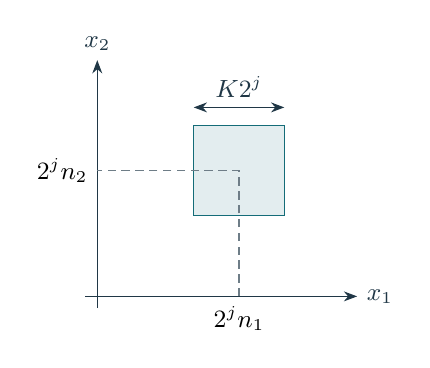
\begin{tikzpicture}[x=1cm,y=1cm,>=Stealth,font=\small]
  \draw[->,ink] (-.15,0)--(3.3,0) node[right] {$x_1$};
  \draw[->,ink] (0,-.15)--(0,3.0) node[above] {$x_2$};
  \filldraw[draw=teal,fill=teal!12] (1.225,1.025) rectangle (2.375,2.175);
  \draw[densely dashed,ink!65] (1.8,0)--(1.8,1.6)--(0,1.6);
  \node[below] at (1.8,0) {$2^j n_1$};
  \node[left] at (0,1.6) {$2^j n_2$};
  \draw[<->,ink] (1.225,2.4)--(2.375,2.4)
    node[midway,above] {$K2^j$};
\end{tikzpicture}
\end{document}
